\documentclass{report}
\usepackage{graphicx} % Required for inserting images
\usepackage[italian]{babel}
\usepackage{tikz}
\usepackage{hyperref}
\usepackage{amsmath}
\usepackage{xcolor}
\usepackage{float}
\usepackage{soul}
\usepackage{listings} % Per evidenziare il codice

\definecolor{lightgray}{rgb}{0.9,0.9,0.9} % Definizione colore sfondo
\definecolor{darkgreen}{rgb}{0.0, 0.5, 0.0}

\lstset{
    backgroundcolor=\color{lightgray}, % Sfondo grigio
    basicstyle=\ttfamily, % Font monospaziato
    % frame=single, % Bordo attorno al codice
    tabsize=4, % Dimensione tabulazione
    breaklines=true, % Permette di andare a capo automaticamente
    numbers = left,
    numberstyle=\small\color{gray}
}

\title{\huge\textbf{{Controllo delle Query Distribuite}}}
\date{Parte III}

\begin{document}

\maketitle
\tableofcontents
\newpage


\chapter{Introduzione}

Torniamo a preoccuparci del problema di confidenzialità, nel contesto di computazione di 
query distribuite; l'assunzione è che non tutti siano autorizzati a vedere tutti i dati, ma ci 
sono dei vincoli di confidenzialità che devono essere rispettati.

\noindent Lo scenario di riferimento è quello in cui ci sono più sorgenti informative, dove 
da un lato ho l'esigenza di condivisione dei dati (per rispondere alle query), mentre dall'altro 
ho esigenza di confidenzialità perché non è detto che chiunque possa leggere i dati.

\section{Join sovrani}
Questo approccio sfrutta la presenza di un hardware fidato (nel senso che nessuno può vedere 
cosa fa), che può ricevere i dati 
per eseguire le computazioni. Lo scenario è:
\begin{itemize}
    \item si hanno due \textit{data owner} che non si fidano l'uno dell'altro
    \item c'è una terza parte, che ha a disposizione dell'hardware fidato, che esegue la computazione
\end{itemize}

\noindent L'idea è che le parti criptano i dati e li mandano all'hardware, che si occupa di:
\begin{itemize}
    \item decriptare i dati 
    \item eseguire la computazione 
    \item recriptare i dati e darli al client 
\end{itemize}

\noindent Un osservatore potrebbe inferire sulla base del risultato qualcosa, come ad esempio 
sulle dimensioni del risultato o sul tempo richiesto ad eseguire la computazione.

\noindent $\Rightarrow$ l'output deve avere più o meno sempre la stessa dimensione e tempo di computazione, 
per cercare di ridurre l'inferenza

\section{Access patterns}
Cercano di specificare come le fonti informative devono essere accedute.

\noindent Definiamo un \textit{access pattern} con un esempio:
\begin{itemize}
    \item abbiamo 3 relazioni, ciascuna con un access pattern, ovvero dei vincoli di accesso
    \item si ha una lettera per ciasuno attributo delle relazione
    \begin{itemize}
        \item $o$ per output 
        \item $i$ per input 
    \end{itemize}

    \begin{figure}[H]
        \centering
        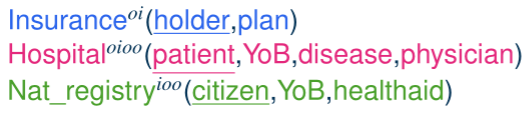
\includegraphics[width=0.6\linewidth]{images/access-pattern.png}
    \end{figure}

    \noindent \textit{per accedere all'attributo "o" mi deve dare l'attributo "i"}; si pongono dei vincoli, 
    l'accesso non è libero
\end{itemize}

\noindent Questa tecnica presenta alcuna svantaggi:
\begin{itemize}
    \item limitata espressione delle limitazioni 
    \item tipicamente ci sono due entità, non un vero scenario distribuito 
    \item può essere difficile da usare nella pratica 
\end{itemize}

\section{Autorizzazioni basate su viste}
La peculiarità di questo approccio è che le restrizioni di accesso dipendono dal contenuto del dato.

\begin{figure}[H]
    \centering
    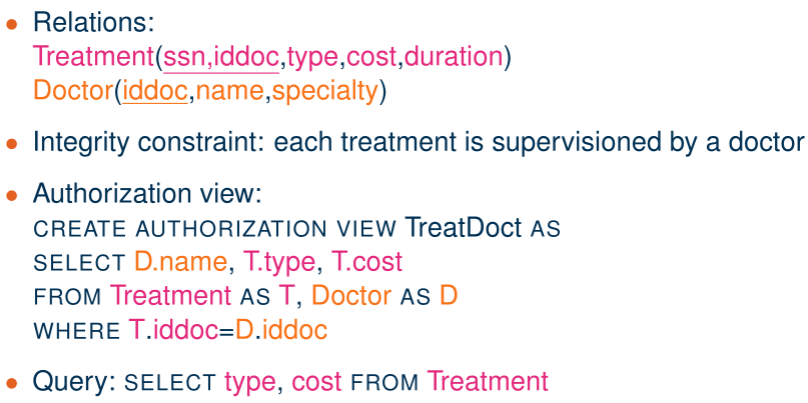
\includegraphics[width=0.8\linewidth]{images/view-auth.png}
\end{figure}

\noindent Verifico se una query può essere eseguita sulla base delle autorizzazioni che 
ho definito; il client scrive la sua query, e il server cerca di rielaborarla 
sulla base delle viste che sono state definite.

\noindent Nel caso in cui una query non possa essere eseguita, ci sono due scenari possibili:
\begin{itemize}
    \item \textit{truman:} ti restituisco un risultato parziale, che corrisponde non alla query che mi hai chiesto ma alla vista che è stata definita (facendotelo 
    passare come completo)
    \item \textit{non-truman:} non ti restituisco nulla e ti dico che non sei autorizzato ad accedere al risultato 
\end{itemize}


\section{Coalition networks}
Ci sono diversi \textit{providers} che si conoscono e che formano delle \textit{coalizioni}; sono 
disposti a condividere le proprie informazioni per un obiettivo comune.

\noindent Ciascun provider ha:
\begin{itemize}
    \item una o più relazioni 
    \item uno o più server
\end{itemize}

\begin{figure}[H]
    \centering
    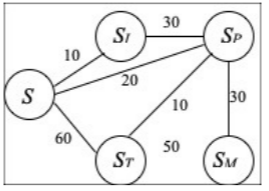
\includegraphics[width=0.4\linewidth]{images/pairwise-auth.png}
\end{figure}

\noindent I server formano una rete, possono comunicare tra di loro; una computazione vuole essere effettuata 
\textbf{minimizzando il costo} (ciascun canale a un costo asssociato) e \textbf{rispettando le restrizioni} 
sul flusso di informazioni (chi può vedere che cosa).


\noindent $\Rightarrow$ Si definisce un \textit{\textbf{safe query plan}}, ovvero un modo per soddsifare la query in modo 
sicuro e che minimizzi i costi:
\begin{itemize}
    \item per le operazioni unarie non ci sono problemi, dato che non richiedono alcun trasferminento di dati 
    \item per le operazioni di join, viene richiesto la cooperazione tra i due server:
    \begin{itemize}
        \item uno funge da \textit{master}, ha il compito di eseguire il join 
        \item uno funge da \textit{slave}, aiuta il master
    \end{itemize}
\end{itemize}

\noindent Dato che l'operazione più costosa e che implica un maggiore flusso di informazioni 
è il join, il \textit{focus} è su come eseguirla in modo da rispettare le autorizzazioni; l'idea che 
sta alla base di questo modello è di supportare diverse operazioni di join in diversi modi, dove 
ognuno di questi implica flussi di informazioni diversi. 

\subsection{Broker join}
Ci sono due relazioni su due server, su cui dobbiamo eseguire il join. Tipicamente, uno 
dei due server funge da \textit{master} e l'altro da \textit{slave}; se però sono state definite delle restrizioni 
che impediscono di accedere all'altra relazione, questa architettura non può esssere utilizzata.

\noindent Con il broker-join si usa (se esiste) un \textbf{terzo server che sia autorizzato ad accedere alle relazioni 
ed eseguire il join}; se ne esiste più di uno, seleziono quello con il costo minore.

\subsection{Peer-join}
Al contrario dello scenario precedente, almeno uno dei due server è autorizzato a leggere 
la relazione dell'altro; il join viene dunque eseguito da uno dei due server (viene scelto quello 
con il costo minore nel caso in cui tutti e due possano farlo).


\subsection{Semi-join}

Entrambi i server entrano in gioco per l'esecuzione dell'operazione di join: 
\begin{itemize}
    \item $S_x$ fa da master, fa una proiezione della sua relazione sull'attributo di join, e la manda a $S_y$
    \item $S_y$ unisce la relazione che ha ricevuto e fa il join con la sua relazione; manda il risultato a $S_x$
    \item $S_x$ completa il risultato aggiungendo gli altri attributi che mancano (dato che inizialmente ha mandato solo l'attributo di join)
\end{itemize}

\subsection{Split-join}

\begin{itemize}
    \item Supponiamo di avere un server $S_x$, con una relazione $r_x = r_{x1} \cup r_{x2}$
    \item Supponiamo, allo stesso modo, di  avere un server $S_y$, con una relazione $r_y = r_{y1} \cup r_{y2}$
    \item Supponiamo che $S_y$ possa accedere solo a una parte di $r_x$, ad esempio solo a $r_{x1}$
    \item Supponiamo, allo stesso modo, che $S_x$ possa accedere solo a una parte di $r_y$, ad esempio solo a $r_{y1}$
\end{itemize}

\noindent $\Rightarrow$ Per rispettare i vincoli di confidenzialità il join viene eseguito in questo modo:
\begin{itemize}
    \item Il server $S_x$ fa il join tra $r_x$ e $r_{y1}$, ovvero ciò a cui può accedere di $r_y$
    \item Il server $S_y$ fa il join tra $r_y$ e $r_{x1}$
    \item A questo punto manca il join tra $r_{x2}$ e $r_{y2}$; nessuno dei due server può leggere 
    questa parte della relazione, per cui viene coinvolta una terza parte che ha l'autorizzazione per farlo 
\end{itemize}

\newpage
\noindent L'operazione di join viene \textit{splittata} in tre parti:
\begin{itemize}
    \item un peer-join svolto da $S_x$
    \item un peer-join svolto da $S_y$
    \item un broker join
\end{itemize}
 

\section{Preferenze in ottimizzazione delle query}

L'aspetto che caratterizza questa classe di soluzioni è che fino ad adesso il \textit{focus} è stato 
lato server; ora si cambia e diventa il client, che vuole eseguire una query, che si preoccupa di come la query viene eseguita 
(magari è sensibile e voglio decidere io come viene svolta).

\noindent Viene modificato il linguaggio che l'utente usa per esprimere la computazione, in modo che 
possa esprimere anche le restrizioni; ad esempio, vediamo due tipi di restrizioni:
\begin{itemize}
    \item \texttt{REQUIRING condition HOLDS OVER $\langle operation, parameters, master \rangle$}
    \begin{itemize}
        \item è un'autorizzazione \textbf{forte}, che deve per forza essere soddisfatta; la restrizione di accesso 
        è \texttt{condition} applicata alle operazioni rappresentate dai nodi della terna, ovvero quelle che 
        riguardano:
        \begin{itemize}
            \item l'operazione $operation$
            \item sugli attributi $parameters$
            \item eseguita da $master$
        \end{itemize}
    \end{itemize}
    \item \texttt{PREFERRING condition HOLDS OVER $\langle operation, parameters, master \rangle$}
    \begin{itemize}
        \item è un'autorizzazione \textbf{debole}, è una preferenza dell'utente; la restrizione applicata segue 
        il ragionamento precedente
    \end{itemize}
\end{itemize}

\noindent In questo modo gli utenti possono definire delle restrizioni su come vengono eseguite le computazioni.




\chapter{Valutazione di query distribuite sotto requisiti di protezione}

\noindent In questo modello si valuta anche il \textbf{bagaglio informativo addizionale} per valutare se una informazione 
può essere trasferita da una parte ad un'altra (ad esempio, una relazione può essere il risultato di una computazione, 
quindi mi sta dando informazioni aggiuntive non esplicite).

\noindent In aggiunta, si usa un modello di autorizzazione che restringe non solo l'informazione che puoi vedere, 
ma anche \textbf{il modo in cui questa informazione può essere computata}.

\noindent $\Rightarrow$ Questi due aspetti sono un qualcosa che i modelli visti in precedenza non considerano

\newpage
\subsubsection{Scenario di riferimento}
Ci sono diverse sorgenti informative; gli archi mostrano come le informazioni possono essere 
combinate tra di loro.

\begin{figure}[H]
    \centering
    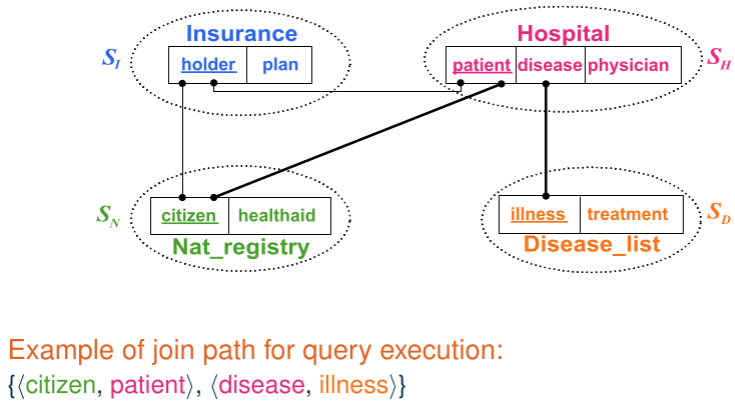
\includegraphics[width=1\linewidth]{images/scenario.png}
\end{figure}


\section{Permessi}
I permessi vengono espressi come una coppia $[Attributes, Join Path] \rightarrow Subject$

$\rightarrow$ \textit{il soggetto è autorizzato ad accedere a tutti gli attributi listati, applicando il join path}

\begin{figure}[H]
    \centering
    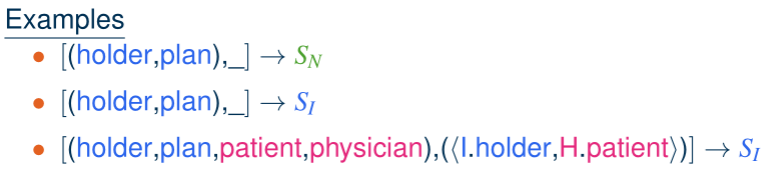
\includegraphics[width=0.8\linewidth]{images/permessi-ex.png}
\end{figure}

\noindent I join path aumentano il potere espressivo, e possono:
\begin{itemize}
    \item Rappresentare \textbf{vincoli di connettività:} stabilisco come sono collegate relazioni diverse
    
    \begin{figure}[H]
        \centering
        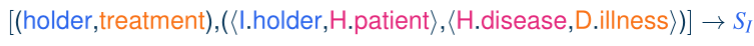
\includegraphics[width=0.8\linewidth]{images/vincoli-conn.png}
    \end{figure}
    \textit{mi dicono come collegare le relazioni affinché questi attributi siano 
    accessibili a un particolare soggetto}
    
    \newpage
    \item Esprimere \textbf{restrizioni sulla quantità di informazioni} a cui un soggetto può accedere 
    
    \begin{figure}[H]
        \centering
        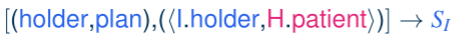
\includegraphics[width=0.5\linewidth]{images/restrizioni.png}
    \end{figure}

    \textit{posso accedere solo alle tuple blu che si uniscono in join alla relazione rosa}

\end{itemize}

\noindent Bisogna fare attenzione al fatto che:
\begin{itemize}
    \item un rilascio di meno tuple (dovuto ad un join path restrittivo) 
    non implica per forza un rilascio di meno informazion
    \begin{figure}[H]
        \centering
        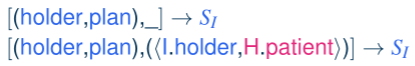
\includegraphics[width=0.5\linewidth]{images/ex1.png}
    \end{figure}
    \item può essere inutile se coinvolge i vincoli di integrità referenziale
    \begin{figure}[H]
        \centering
        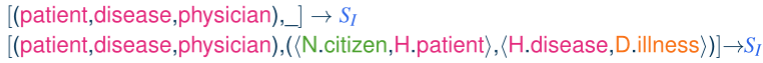
\includegraphics[width=0.9\linewidth]{images/ex2.png}
    \end{figure}
\end{itemize} 

\section{Profilo della relazione}
È un concetto che cerca di catturare il concetto di informazione aggiuntiva non esplicita;
il \textbf{profilo di una relazione} è una tripla $[R^\pi, R^{\bowtie}, R^\sigma]$, dove:
\begin{itemize}
    \item $R^\pi$ è la relazione esplicita
    \item $R^{\bowtie}$ è il join path eseguito per ottenere la relazione $R$
    \begin{itemize}
        \item \textit{come ho ottenuto questa relazione? è stata ottenuta da un join?}
    \end{itemize}
    \item $R^\sigma$ è il set di attributi che sono stati coinvolti in operazioni di selezioni 
    applicate per ottenere la relazione $R$
    \begin{itemize}
        \item \textit{R deriva da qualche condizione applicata su attributi che non sono esplicitamente presenti nella relazione?}
    \end{itemize}
\end{itemize}

\subsubsection{Esempio}

\begin{figure}[H]
    \centering
    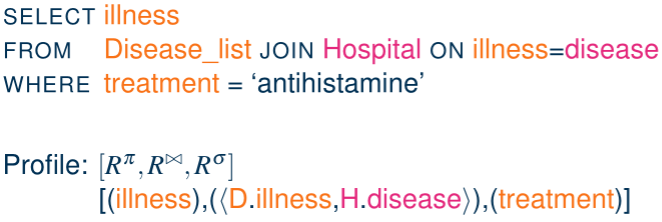
\includegraphics[width=0.7\linewidth]{images/relation-profile-ex.png}
\end{figure}

\section{Vista autorizzata}

Un soggetto $S$ è autorizzato ad accedere ad una vista $R$ sse:

\noindent \hl{ $\exists [Attributes, Join Path]
\rightarrow S | R^\pi \cup R^\sigma \subseteq Attributes \wedge  R^{\bowtie} = Join Path$}

\noindent $\Rightarrow$ \textit{Un soggeto è autorizzato ad accedere ad una relazione quando:
\begin{itemize}
    \item tutti gli attributi espliciti e quelli che usati per definere le condizioni che hanno 
    ristretto le tuple che fanno parte della relazione, sono attributi a cui il soggetto può accedere
    \item il join nella componente R deve essere uguale al join path a cui il soggetto è autorizzato; devono essere ottenuti in quel 
    modo, altrimenti sta accedendo ad informazioni a cui non ha diritto ad accedere
\end{itemize}
}

\begin{figure}[H]
    \centering
    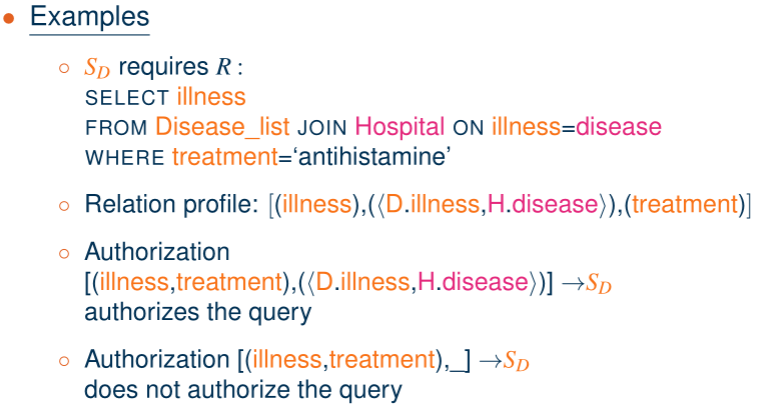
\includegraphics[width=0.8\linewidth]{images/auth-view-ex.png}
\end{figure}

\section{Rilasci autorizzati}
Devo trovare un modo per eseguire la computazione in modo che rispetti i vincoli del sistema.
Le operazioni si dividono in:
\begin{itemize}
    \item \textbf{Unarie}; possono essere eseguite dal server $S$ che tiene la relazione
    \begin{itemize}
        \item proiezione: $\pi_X(R)$
        \item selezione: $\sigma_X(R)$
    \end{itemize}
    \item Operazioni di \textbf{join}; possono essere eseguite solo se implicano il rilascio 
    di \textit{viste autorizzate}. Si possono usare due strategie per eseguire il join soddisfando le autorizzazioni:
    \begin{itemize}
        \item Regular join (master e slave) 
        \begin{figure}[H]
            \centering
            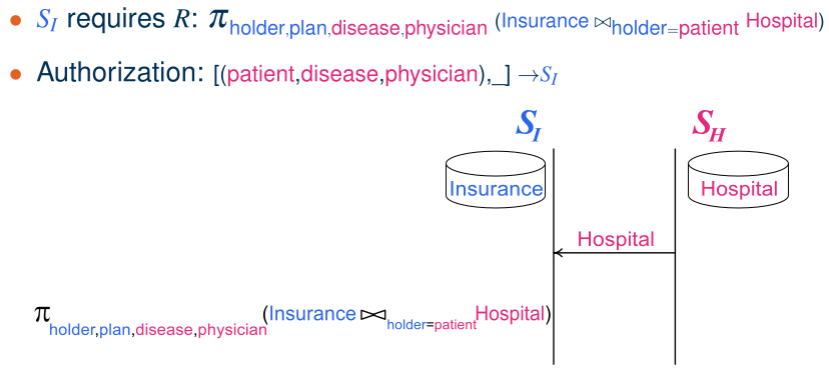
\includegraphics[width=1\linewidth]{images/regular-join.png}
        \end{figure}

        \item Semi-join
        \begin{figure}[H]
            \centering
            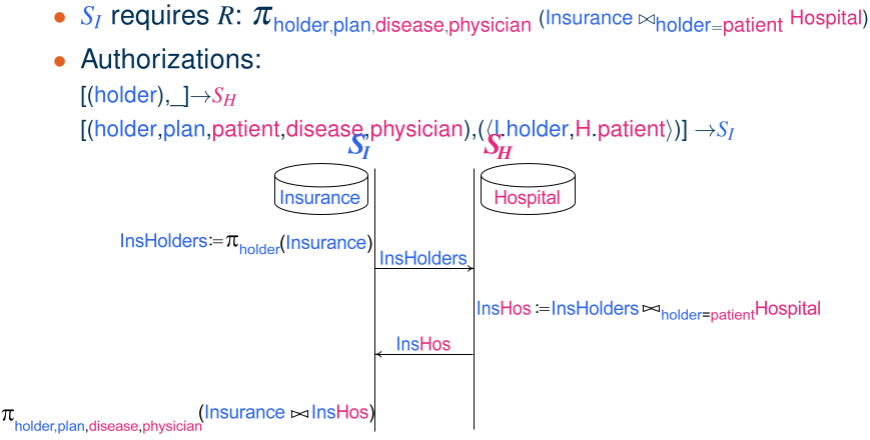
\includegraphics[width=1\linewidth]{images/semi-join.png}
        \end{figure}
    \end{itemize}
 \end{itemize}


\section{Algoritmo}
Data la computazione che voglio eseguire e dato l'insieme di autorizzazioni, l'obiettivo 
è quello di calcolare come eseguire la computazione in modo da rispettare le autorizzazioni.

\noindent L'idea è di fare l'assegnamento in due passi:
\begin{enumerate}
    \item Cerco tutti i soggetti che sono potenzialmente autorizzati ad eseguire una operazione 
    \begin{itemize}
        \item faccio una visita post-order dell'albero (L, R, root; in pratica dalle foglie risalgo) 
    \end{itemize}
    \item Faccio una visita in pre-order dell'albero e ne scelgo uno; può essere fatta in diversi modi in base a qual è il parametro di voglio ottimizzare
\end{enumerate}

\section{Sintassi vs Semantica}

\begin{figure}[H]
    \centering
    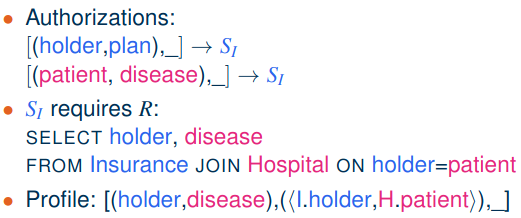
\includegraphics[width=0.7\linewidth]{images/sintassi-semantica.png}
\end{figure}

Per vedere se il server è abilitato ad accedere al risultato della query, devo vedere qual è il contenuto informativo associato 
alla query, ovvero il suo profilo.

\noindent Devo vedere se le autorizzazioni del sistema coprono il profilo della query: quello che vediamo è che non c'è una autorizzazione 
esplicita che permette di effetuare il join e di accedere a quella particolare query; tuttavia, ha più permessi che composti tra loro permettono 
di accedere al medesimo risultato.

\noindent Se mi va bene avere più autorizzazioni che composte tra loro permettono di accedere allo stesso risultato, è un tipo di approccio \textbf{semantico}.

\noindent Se voglio che ci sia una autorizzazione esplicita fatta in modo preciso è un tipo di approccio \textbf{sintattico}.


\chapter{Composizione di autorizzazioni}
Facciamo diverse assunzioni:
\begin{itemize}
    \item lo schema è privo di cicli 
    \item consideriamo solo join di tipo \textit{naturale}; se c'è un informazione che è presente in più relazioni, allora supponiamo 
    che usi sempre lo stesso nome (esempio SSN)
    \item Le composizioni vengono definite sempre per \textit{stesso soggetto}, diventa una semplice coppia $[Attr, Rel]$
    \item Il profilo della relazione $[R^\pi, R^{\bowtie}, R^\sigma]$ viene semplificato come $[Attr, Rel]$ dove:
    \begin{itemize}
        \item $Attr = R^\pi \cup R^\sigma$
        \item $Rel$ sono le relazioni coinvolte nel join path $R^{\bowtie}$ (mi basta specificare che il join lega due relazioni, senza specificare 
        su quali il attributo perché abbiamo supposto di avere \textit{join naturali})
    \end{itemize}
\end{itemize}

\section{\textit{Schema graph}}
Conviene rappresentare attraverso un grafo lo schema per capire meglio quando è \textit{safe} comporre delle autorizzazioni.

\noindent Un \textit{grafo di schema} a partire da un set di relazioni è un grafo misto dove:
\begin{itemize}
    \item ci sono tanti nodi quanti sono gli \textbf{attributi} delle relazioni
    \item ci sono degli \textbf{archi orientati} che rappresentano le \textbf{dipendenze funzionali} da una chiave verso tutti gli altri attributi della medesima relazione
    \item ci sono degli \textbf{archi orientati} che rappresentano i vincoli di \textbf{integrità referenziale}
    \item ci sono \textbf{archi non orientati} che rappresentano le operazioni di \textbf{join}
\end{itemize}

\begin{figure}[H]
    \centering
    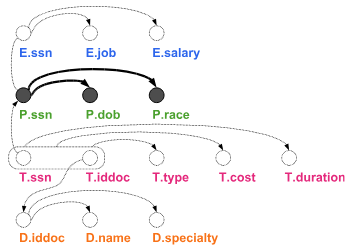
\includegraphics[width=0.7\linewidth]{images/view-graph.png}
\end{figure}

\section{\textit{Views}}

Permessi e query $[Attr, Rel]$ sono una \textbf{vista} su un set di relazioni $R$ del mio sistema, dove 
il contenuto informativo di questa vista non cambia se viene estesa andando a chiuderla usando i vincoli di integrità referenziale; si definisce 
un \textit{insieme di chiusura di relazione} ottenuto seguendo i vincoli di integrità referenziale a partire da una relazione.

\section{\textit{View Graph}}
Una vista può essere rappresentata graficamente attraverso una colorazione dello \textit{schema graph}; viene colorata la porzione del grafo che corrisponde 
di una vista $[Attr, Rel]$ nel seguente modo:
\begin{itemize}
    \item di nero gli attributi che compaiono esplicitamente in $Attr$
    \item di nero tutti gli archi che corrispondono al join path definito sull'insieme di chiusura di $Rel$, oppure gli archi che partono 
    da una chiave e vanno versi attributi neri
    \item di bianco tutti gli attributi che non sono neri della chiusura di $Rel$ e gli archi che li connettono alla chiave primaria
    \item \textit{clear} per tutti gli altri attributi e archi (un terzo colore)
\end{itemize}

\begin{figure}[H]
    \centering
    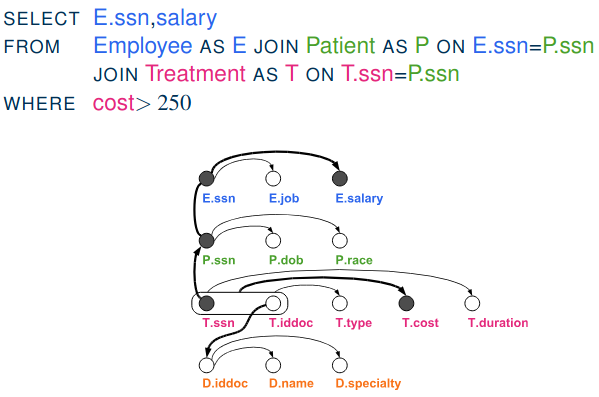
\includegraphics[width=1\linewidth]{images/view-graph2.png}
\end{figure}

\noindent In figura la vista del risultato è $[(ssn, salary, cost), (Employee, Patient, Treatment)]$


\section{Autorizzare le query}
Un soggetto vuole eseguire una query; il sistema deve controllare se il soggetto è autorizzato ad accedere al risultato della query; se 
non può accedervi, la query non viene neanche eseguita.

\noindent Ho da una parte il profilo della query e dall'altra la vista dei permessi; devo prima vedere quando una autorizzazioni si applica alla query (quando 
riguarda le stesse informazioni che ti sto chiedendo), e vedo se mi danno il permesso di accedere al risultato:

\begin{itemize}
    \item $p = [Attr_p, Rel_p]$ si \textbf{applica} a $q = [Attr_q, Rel_q]$ sse $Rel^*_p \subseteq Rel^*_q$
    \item $p = [Attr_p, Rel_p]$ \textbf{autorizza} a $q = [Attr_q, Rel_q]$ sse:
    \begin{itemize}
        \item $p$ si applica a $q$
        \item $G_q$ e $G_p$ hanno gli \textbf{stesso} archi neri di integrità referenziale e join
        \item tutti i nodi che sono neri $G_q$ lo sono anche in $G_p$
    \end{itemize}

    $\rightarrow$ devo sostanzialmente vedere che tutto ciò che è nero nella query lo è anche nei miei permessi, sia archi che nodi
\end{itemize}

\subsection{Esempi}

\begin{figure}[H]
    \centering
    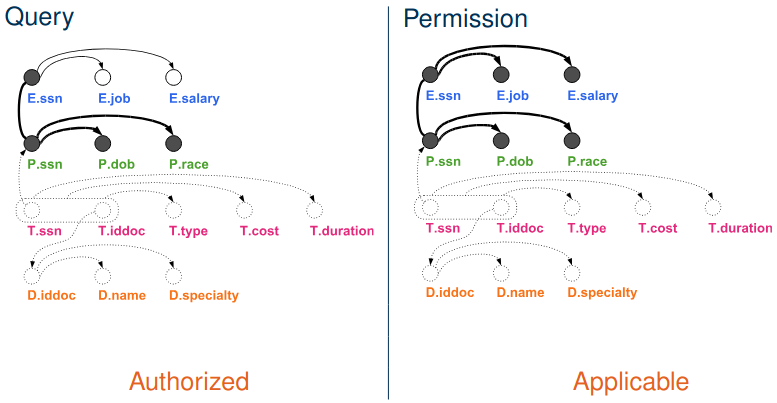
\includegraphics[width=1\linewidth]{images/perm1.png}
\end{figure}

\begin{figure}[H]
    \centering
    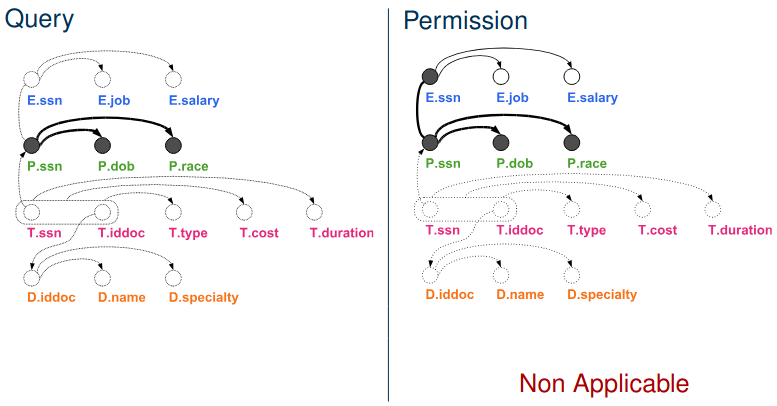
\includegraphics[width=1\linewidth]{images/perm2.png}
\end{figure}

\noindent $Rel^*_p = \{E, P\}$, mentre $Rel^*_q = \{P\}$. 

\noindent Non posso applicare questo permesso perché c'è il join, mi 
porta un contenuto informativo maggiore che non c'è nella query. 
\noindent Il permesso mi dice \textit{tutti i pazienti che sono anche impiegati}; la query mi dice \textit{tutti i pazienti}. Me ne accorgo perché 
ci sono delle operazioni di join che nella query non ci sono, che mi danno delle informazioni in più (e allo stesso mi toglie).

\begin{figure}[H]
    \centering
    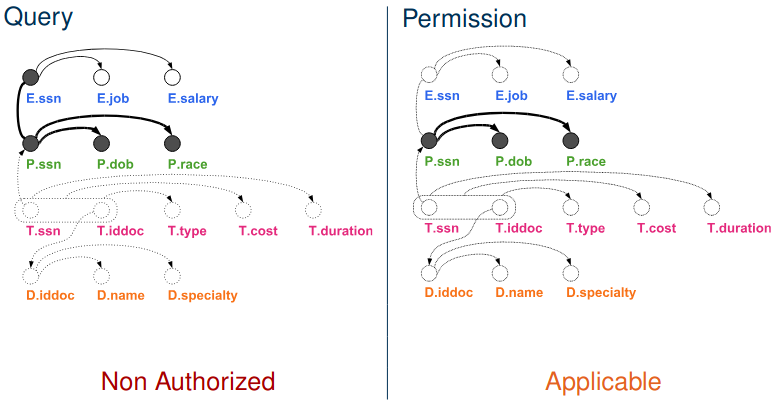
\includegraphics[width=1\linewidth]{images/perm3.png}
\end{figure}

\section{Composizione di permessi}
Questo modello mi permette di applicare un approccio semantico; posso avere più permessi che mi vanno 
a coprire la query che mi permettono di accedere al risultato.

\noindent Una query può essere eseguita se il soggetto ha i permessi per vedere il contenuto informativo della query; una query dovrebbe essere 
autorizzata se il soggetto ha i permessi per computare in modo indipendente il risultato.

\noindent Un singolo permesso potrebbe non essere sufficiente, dunque si usa la \textbf{composizione} di permessi. Bisogna fare attenzione
al rischio di \textit{disclosure indiretta}.

\subsection{Esempi}

\begin{figure}[H]
    \centering
    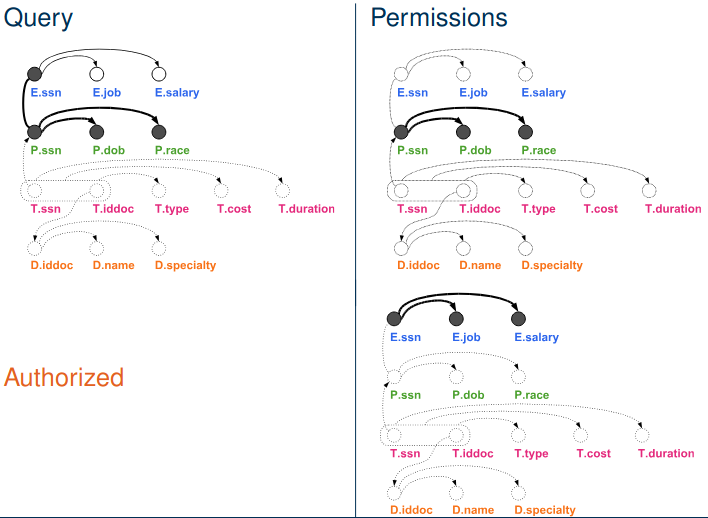
\includegraphics[width=1\linewidth]{images/comp1.png}
\end{figure}

\begin{figure}[H]
    \centering
    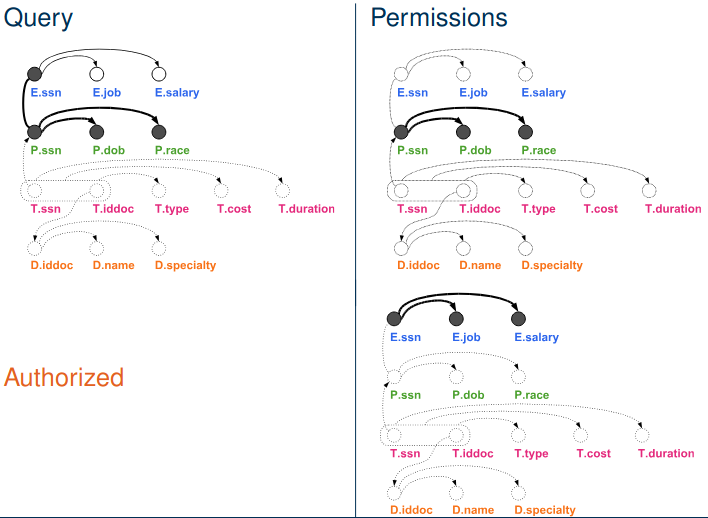
\includegraphics[width=1\linewidth]{images/comp1.png}
\end{figure}

\noindent Potremmo fare il ragionamento di \textit{sovrapporre} i permessi: avremmo tutto ciò che ci serve colorato di nero, e potremmo 
pensare di essere autorizzati ad accedere alla query.

\noindent Tuttavia, questa composizione non può essere fatta perché manca l'associazione tra $SSN$ (un paziente specifico) e $specialty$; anche eseguendo 
singolarmente le computazioni non rieco a ricostruire il risultato della query.

\section{Composizione sicura}
Due permessi possono essere composti in maniera \textbf{sicura} sse la loro composizione \textbf{non aggiunge informazione}.
\begin{itemize}
    \item $p_i \rightarrow p_j$: $p_j = [Attr_j, Rel_l]$ dipende da $p_i = [Attr_i, Rel_i]$ sse l'intersezione degli insiemi di attributi 
    $Attr_i$ e $Attr_j$ è un insiemi di attributi tutti neri in $p_j$, e a partire da questi attributi ci deve essere un cammino (in uno dei due grafi)
    che mi permette di raggiungere tutti gli altri nodi neri attraversando solo archi neri

    $\Rightarrow$ se è verificato posso comporre i permessi
\end{itemize}

\subsection{Esempi}

\begin{figure}[H]
    \centering
    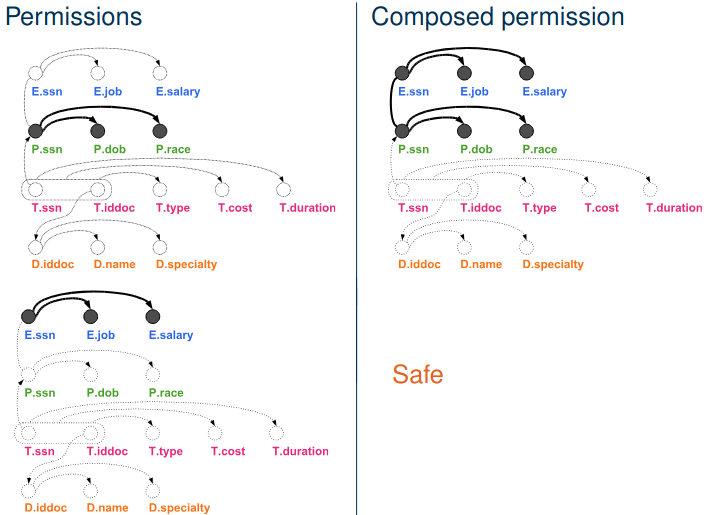
\includegraphics[width=1\linewidth]{images/safe1.png}
\end{figure}

\begin{figure}[H]
    \centering
    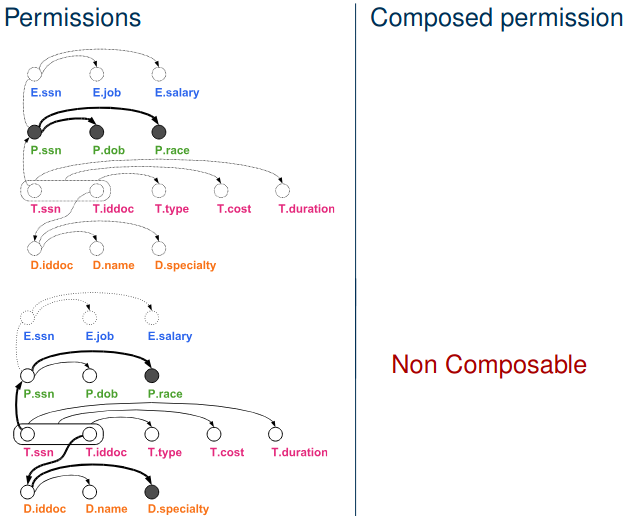
\includegraphics[width=1\linewidth]{images/safe2.png}
\end{figure}

\section{Esecuzione di Access Control}
Data una query, come faccio a vedere se è può essere autorizzata oppure no? Il processo richiede tre passi:
\begin{enumerate}
    \item determino tutti i permessi applicabili alla query 
    \item determino tutti i permessi che ottengo attraverso il processo di composizione (fino a a quando termina; quando compongo un permesso allo 
    stesso tempo uno viene tolto dall'insieme, per cui a una certa il processo termina)
    \item guardo se esiste un permesso (tra quelli esistenti e quelli che ho ottenuto con la composizione) che copre la query che voglio eseguire 
\end{enumerate}

\noindent L'efficienza garantita dallo sfruttamento dell'implicazione dei permessi:
\begin{itemize}
    \item Se \textit{$p_j$} $\rightarrow$ \textit{$p_i$}, $\forall p_k \in P$:
    \begin{itemize}
        \item  $ p_j \rightarrow p_k \Rightarrow ( p_i \otimes p_j) \rightarrow p_k$
        \item  $ p_k \rightarrow p_j \Rightarrow p_k \rightarrow (p_i \otimes p_j)$
        
        
        $\rightarrow$  aggiungendo $ p_i \otimes p_j, p_j$ può essere rimosso da P
    \end{itemize}
    \item Non c'è necessità di computare tutte le $2^n - 1$ composizioni di \textit{n} permessi
    \item La complessità computazionale rimane polinomiale ossia \textit{O}($n^3$)
\end{itemize}

\noindent \textbf{Spieghino della prof:} Supponiamo di avere tre permessi, $p_i ,p_j$ e $p_k$ quello che osseravo è che $p_i$ e $p_j$
sono due autorizzazioni che possono essere composte tra di loro perchè $p_i$ dipende da $p_j$. Se $p_i$ e $p_j$ sono componibili tar di loro
e se esiste un'altra autorizzazione $p_k$ tale per cui $p_k$ dpende da $p_j$ allora in pratica $p_j$ si può buttar via, tanto $p_k$ dipende dal
risultato della composizione tra $p_i$ e $p_j$.
Questo è vero non solo quando $p_k$ dipende da $p_j$ ma anche quando $p_j$ dipende da $p_k$, in ogni caso io $p_j$ posso buttarlo via senza perdere nulla.

\noindent \textbf{N.B. :} La prof ha fatto degli esercizi su sta cosa 

\chapter{Un modello di autorizzazione per query multi-provider}

Normalmente un modello di autorizzazione è binario, nel senso che puoi accedere all'informazione oppure no; la peculiarità del modello 
che adesso vediamo è che aggiunge un \textit{terzo livello di visibilità}:
\begin{itemize}
    \item puoi accedere ai dati
    \item non puoi accedere ai dati
    \item puoi accedere ai dati criptati 
\end{itemize}

\noindent Il vantaggio è che potrebbe essere conveniente in termini economici, usando magari server poco fidati.

\section{Definizione del problema}

\begin{itemize}
    \item \textbf{INPUT:}
    \begin{itemize}
        \item Query 
        \item Set di cloud providers, ciascuno con le sue informazioni che sono messe a disposizione per poter eseguire le query in modo collaborativo
        \item Specifica di autorizzazioni 
    \end{itemize}
    \item \textbf{OUTPUT:}
    \begin{itemize}
        \item Assegnare le operazioni ai soggetti in modo da soddisfare le autorizzazioni (che ciascun soggetto ha definito sui propri dati) e minimizzare i costi
    \end{itemize}
\end{itemize}

\noindent L'idea è di dare l'autorizzazione a un soggetto di eseguire delle operazioni no sui dati in chiaro ma sui dati cifrati,
può essere conveniente quando mi fido di un soggetto ma non troppo.


\section{Profilo della relazione}
È il bagaglio informativo della relazione;no solo inteso come attributi della relazione ma anche altre informazioni che non appaiono in modo esplicito, deve essere adattato a questo modello ed include tre componenti:
\begin{itemize}
    \item $v$: attributi espliciti dello schema della relazione, sia in chiaro che in forma criptata (devo distinguere queste due situazioni)
    \begin{itemize}
        \item prima erano $R^\pi$
    \end{itemize}
    \item $i$: attributi impliciti (per costruire la relazione ho usato delle condizioni su attributi in chiaro o criptati), sia in chiaro che in forma criptata (devo distinguere queste due situazioni), le informazioni che io vedo dipendono in qualche modo da questi attributi su cui io ho applicato dterminate condizioni.
    
    \begin{itemize}
        \item \textbf{Selection:} faccio una selezione dove scelgo in base alla peculiarità di un determinato altro attributo, creo un collegamento con l'attributo peculiare anche se non fa parte dello schema
        \item \textbf{Grouping:} selezione facendo raggruppamento 
    \end{itemize}
    \begin{itemize}
        \item prima erano $R^\sigma$
    \end{itemize}
    \item $\simeq$: ho gli attributi coinvolti in operazioni di join (si suppone join naturali, prima erano $R^{\bowtie}$)
    \begin{itemize}
        \item \textbf{Comparing} attributes: facciamo un confronto ad esempio $S=C$, se io confronto questi attributi e mettiamo caso che per l'utente lattributo $S$ debba essere criptato, essendo un'equivalenza basta poter vedere $C$ per conoscere anche $S$ che però non ho l'autorizzazione per conoscere.
        
        \noindent Per ovviare a questo problema se si deve dare questa relazione a un soggetto questo soggetto può ricevere la relazione solo se è abilitato a vedere $S$ e $C$ allo stesso modo.
    \end{itemize}
\end{itemize}

\section{profili risultanti dalle operazioni}
\begin{figure}[H]
    \centering
    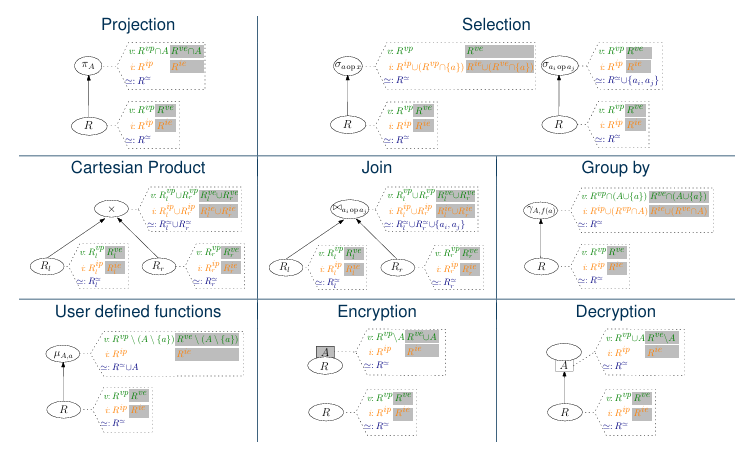
\includegraphics[width=1\linewidth]{images/risultatiOperazioni.png}
\end{figure}

\noindent Tutti gli esempi sono organizzati nello stesso modo: a sx il modo generale a dx un'esempio. 
\subsection{Proiezione}
Se io parto da una relazione R che ha questi profilo ed eseguo una proiezione, la relazione risultato ha lo stesso profilo, l'unica cosa che cambia sono gli attributi \textbf{visibili}.  
\begin{itemize}
    \item Esempio: nella relazione la proieizione viene fatta su $B$ e su $P$ butto via $D$ e $T$.
\end{itemize}

\subsection{Selezione - 1}
Selezione $=$ io vado ad eseguire una condizione su determinati attributi. Viene fatta una distinzione su qual è la forma della condizione:
se la condizione è $attributo = valore$ mi devo ricordare che è stata eseguita quella condizoone su quell'attributo, quindi quell'attributo deve finire nella componente implicita del profilo della mia relazione.
\begin{itemize}
    \item Esempio: Se io faccio "D$=$stroke" allora poi l'attributo D dovrà finire nella componente implicita
\end{itemize} 

\subsection{Selection - 2}
In questo caso nella selezione vengono comparati due attributi (e non attributo con valore), ha effetto sul campo delle equivalenze
\begin{itemize}
    \item Esempio: SC viene aggiunto al campo equivalenze
\end{itemize}

\subsection{Prodotto cartesiano}
Quando viene fatto il prodotto cartesiano tra due relazioni devo unire i profili delle relazioni
\begin{itemize}
    \item Esempio: si uniscono tutti i campi delle due relazioni
\end{itemize}

\subsection{Join}
Vuol dire ancora una volta che devo fare l'unione dei due profili, è simile al prodotto cartesiano 
\begin{itemize}
    \item Esempio: in questo caso mi devo ricordare che oltre a unire i profili ho anche confrontato gli attributi $D$ e $C$ e questo va aggiunto nella componente delle equivalenze 
\end{itemize}


\subsection{Group by}
Raggruppo le tuple della mia relazione in base a uno o più attributi,e su questi gruppi posso eseguire delle funzioni di aggregazione.
\begin{itemize}
    \item Esempio: in questo caso average(AVG) viene applicato alla relazione, io ottengo una nuova relazione che ha come schema l'attributo T e quello che ho come secondo attributo
    non è proprio l'attributo P, ma è il risultato di una funzione che io ho applicato all'attributo P. 
    Devo ricordarmi di aggiungere l'attributo T negli attributi impliciti della mia relazione, a livello di equivalenza invece non cambia nulla.
\end{itemize}

\subsection{Funzioni definite dall'utente}
Sono delle funziomi che io posso avere all'interno delle query SQL tipo machine learning, io non so di preciso questa funzione.
\begin{itemize}
    \item Esempio: cambia lo schema degli attributi visibili, è una funzione UDF che in una coppa $(S,B)$ prende solo l'attributo $S$.
    Fondamentalmente sparisce l'attributo $B$, nella classe delle equivalenze viene fatta l'unione tra SC già presenti e SB confrontati ora e ottengo SBC.
\end{itemize}


\subsection{Encryption}
Se cripto un attributo in una relazione, quell'attributo sarà ancora parte della relazione però criptato.

\subsection{Decryption}
Se decripto un attributo, poi lo vedo in chiaro.

\section{Visibilità autorizzata}
\begin{figure}[H]
    \centering
    \includegraphics[width=1\linewidth]{images/visibilità autorizzata.png}
\end{figure}

Introduciamo il concetto con un esempio: Ummaginiamo di avere sempre le nostre due relazinoi Hospital e Insurance. Nella tabella vediamo rappresentate
le autorizzazioni definite su queste due relazioni per i vari soggetti all'interno del sistema.

\noindent $H$ sta per Hospital ed è il proprietario della relazione Hospital, $I$ sta per Insurance ed il proprietario della relazione insurance,
poi abbiamo altri soggetti, in questo esempio $U$ è l'utente che richiede la computazione.

\noindent A sx R è la relazione che è il risultato di una query.

\noindent Data questa relazione e questa tabella andiamo a vedere chi è autorizzato ad accedere alla relazione R:
Intuitivamente un soggetto è autorizzato ad accedere alla relazione R se può accedere in chairo a tutti gli attributi che sono in chairo nella relazione e può accedere agli attributi
che appaiono in forma criptata o in chairo o in modalità criptata (questo per quanto rguarda gli attributi nei campi $v$ e $i$). Per wuanto riguarda il campo delle equivalenze un soggetto
deve avere una visibilità uniforme su questi attributi.
\begin{itemize}
    \item \textbf{Soggetto H:} il soggetto $H$ ha una visibilità criptata sull'attributo $P$ quindi non può accedere alla relazione 
    \item \textbf{Soggetto I:} il soggetto $I$ è okay per gli attributi visibili  ma non ha visibilità uniforme sulle equivalenze poichè $S$ è criptato e $C$ in chiaro, quindi non è autorizzato ad accedere 
    \item \textbf{Soggeto U:} non ha accesso all'attributo $B$, quini non è autorizzato
    \item \textbf{Soggetto X:} visibilità criptata su $P$ quini no accesso
    \item \textbf{Soggetto Y:} può accedere.
    \item \textbf{Soggetto Z:} visibilità criptata su $P$ quini no accesso
\end{itemize} 

\noindent In conclusione:

\noindent \textit{Un soggetto S è autorizzato ad accedere alla relazione R se:}
\begin{itemize}
    \item visibilità del testo in chiaro su attributi in chiaro (visibili o impliciti)
    \item visibilità in chairo o criptata su attributi criptati (visibili o impliciti)
    \item visibilità uniforme (in chiaro o criptata) su attributi equivalenti
\end{itemize}


\section{Calcolo delle assegnazioni}
\begin{figure}[H]
    \centering
    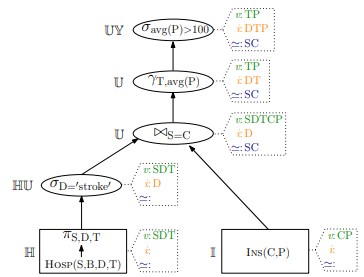
\includegraphics[width=0.6\linewidth]{images/calcoloassegnazioni.png}
\end{figure}

Parto da una situazione dove tutto è in chairo e guardo chi può eseguire le varie operazioni di cui la mia query si compone. Partiamo 
dalle foglie e andiamo verso l'alto, abbiamo sempre le nostre due relazioni Hospital e Insurance, di base queste due relazioni
possono essere gestite da H per Hospital e I per Insurance.
\begin{itemize}
    \item Analizzando la query è visibile come nella relazione Hospital l'attributo $B$ non è mai coinvolto all'interno della computazione,
quindi viene fatta una \textbf{proiezione}, rappresentata con $\pi$, non le rappresento con un nodo dell'albero poichè rientra tra le cose che può fare
chi ha in mano la relazione.
    \item Andiamo sul nodo sopra con l'operazione di \textbf{selezione} su $D$, visto che l'idea è lasciare tutto in chiaro vado a vedere chi è autorizzato a vedere in chiaro la relazione $H$ che contiene
al suo interno gli attributi $S$ , $D$ e $T$. Guardando la tabella notiamo che solo gli utenti $H$ e $U$ sono autorizzati a vedere questi attributi in chairo.
    \item Arrivo al nodo di join, l'unico soggetto che può vedere la relazione che da una parte ha gli attributi $SDT$ in chairo e gli attributi $CP$ dell'altra relazione in chairo è solo il soggetto $U$
    \item Questo ragionamento è valido anche per tutti gli altri nodi, notiamo che però se lasciamo tutto in chairo ogni nodo è caratterizzato da pochi candidati.  
\end{itemize}

\noindent Faccio l'opposto e parto dall'assunzione che sia \textbf{tutto criptato} (guardare immagine sotto)
\begin{figure}[H]
    \centering
    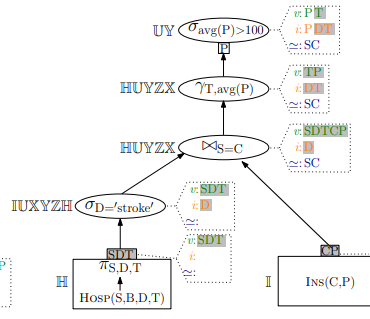
\includegraphics[width=0.6\linewidth]{images/cal2.png}
\end{figure}

\noindent Supporre di avere tutto criptato aumenta notevollmente il numero di candidati, infatti nella realtà non è detto che sia tutto criptato bensì
è solo una strategia che applico per trovare i candidati.
In questa query c'è un assunzione particolare: la $P$ che si trova sotto l'ultimo nodo dell'albero (quello più in alto) indica l'\textbf{operazione di decriptazione},
viene fatto poichè determinate operazioni vogliono essere eseguite sugli attributi in chairo. Il valore che dipende dall'attributo $P$ deve essere decriptato.

\section{Piano di query minimamente esteso}
\begin{figure}[H]
    \centering
    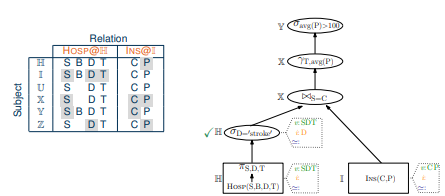
\includegraphics[width=0.8\linewidth]{images/minimal.png}
\end{figure}

In qualche modo abbiamo applicato un qualche criterio e questi sono i soggetti che abbiamo scelto.
\begin{itemize}
    \item Il soggetto $H$ deve compiere l'operazione di selezione su D, e al fine che la possa compiere io devo lasciare tutto così com'è e non criptare nulla.
    \item Per l'operazione di Join abbiamo scelto il soggetto $X$, però può accedere gli attributi solo in modalità criptata. Quindi quando vado ad eseguire la query devo iniettare delle operazioni di \textbf{criptazione} (tutto questo dipende dal sogetto che scelgo per fare una determinata operazione)
    \begin{figure}[H]
    \centering
    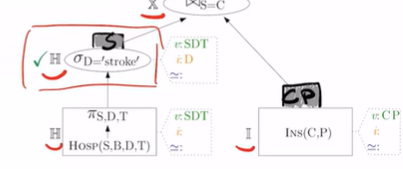
\includegraphics[width=0.4\linewidth]{images/onthefly.png}
\end{figure}
    \item L'operazione successiva la svolge sempre $X$ che consegna il risultato al soggetto $Y$, l'operazione che $Y$ deve fare va eseguita in chiaro
    sull'attributo $P$ che però il soggetto $X$ ha criptato, quindi decripta l'attributo $P$ prima di svolgere l'operazione.
\end{itemize}

\noindent Scherma finale risultante:
\begin{figure}[H]
    \centering
    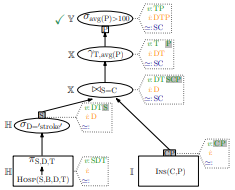
\includegraphics[width=0.4\linewidth]{images/min2.png}
\end{figure}

 \noindent \textbf{Problema della gestione delle chiavi di criptazione:} chiavi che devono essere condivisi tra più soggetti, quelli che eseguiranno 
l'operazione. 


\end{document}
